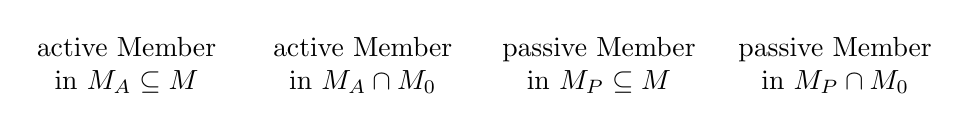
\begin{tikzpicture}
    \activeMember{foo}{(0,0)}{\phantom{/}…\phantom{/}}
    \node [align=center] at (0,-1.8) {active Member\\in $M_A \subseteq M$};
    \activeMember{foo}{(3,0)}{\phantom{/}\ul{…}\phantom{/}} % causal
    \node [align=center] at (3,-1.8) {active Member\\in $M_A \cap M_0$};
    \passiveMember{foo}{(6,0)}{\phantom{/}…\phantom{/}}
    \node [align=center] at (6,-1.8) {passive Member\\in $M_P \subseteq M$};
    \passiveMember{foo}{(9,0)}{\phantom{/}\ul{…}\phantom{/}} % causal
    \node [align=center] at (9,-1.8) {passive Member\\in $M_P \cap M_0$};
\end{tikzpicture}